\chapter*{Introduction}
\addcontentsline{toc}{chapter}{Introduction}
\label{chap:Intro}
Ce document a été réalisé dans le cadre du bureau d'étude du module "Conception et intégration des systèmes critiques" qui a pour sujet la conception à l'aide d'UML 2.0 et SysML d'un système de robot planteur.
La mission principale du robot est de planter des légumes (choux, salades) sur des planches reparties dans une parcelle de culture défini comme suis :\\%
 \begin{figure}[!ht]
 \centering
 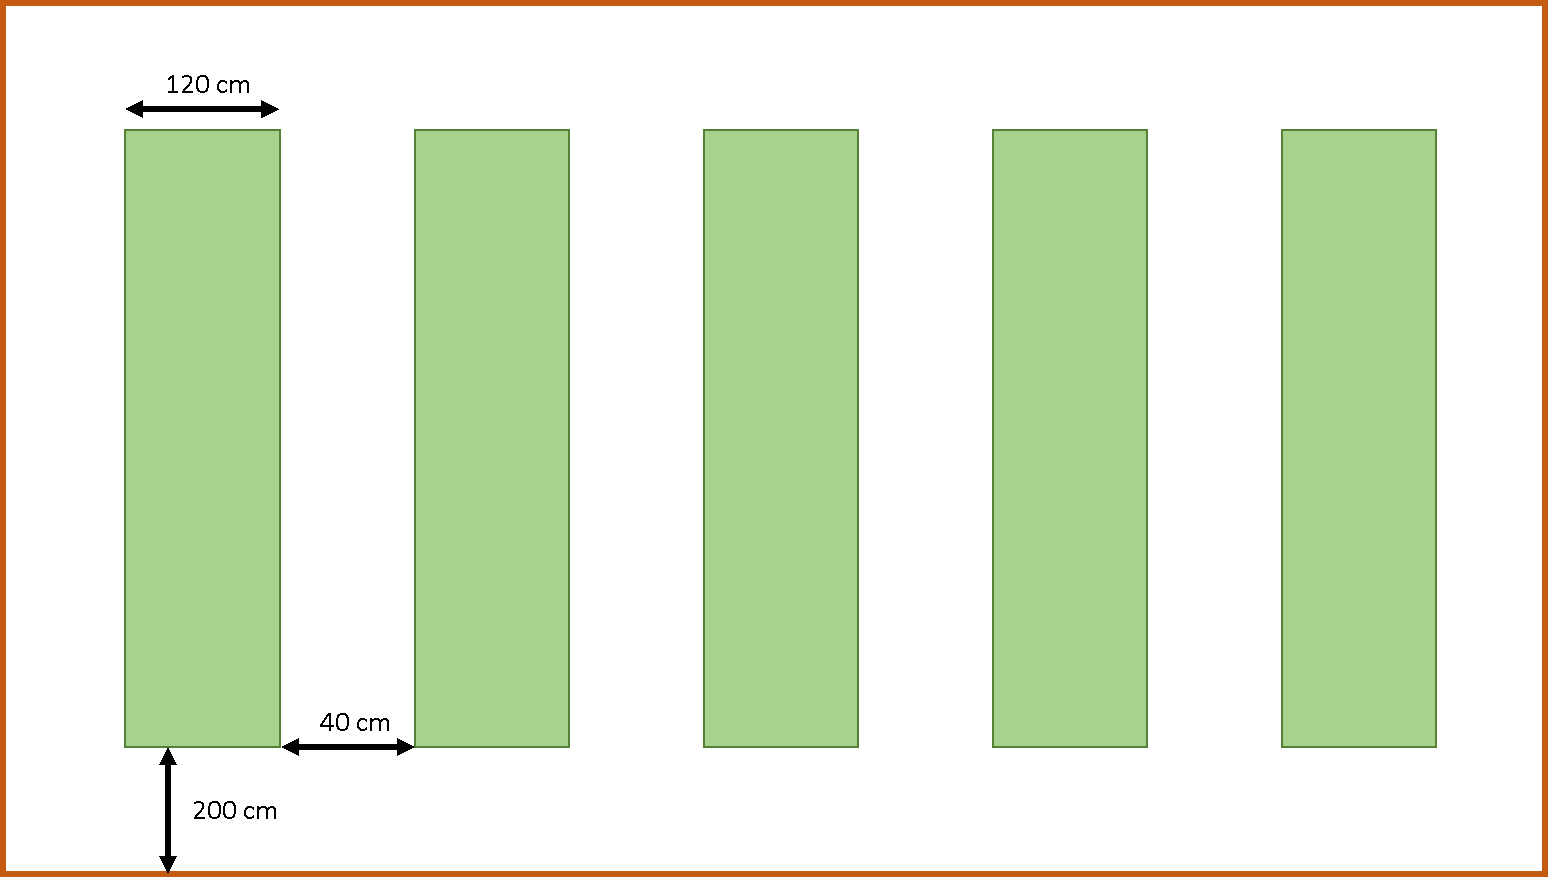
\includegraphics[width = .7\textwidth]{./introduction/champs_planches.png}
 \caption{Schéma d'un champ à 5 planches.}
 \end{figure}


Une parcelle est composée de planches de 1m20 de large et de hauteur inférieure à 50 cm délimitées sur la longueur par des passes pieds de 40 cm de large. De part et d'autres des planches, en largeur, se trouve une cornière de 2m.
La partie analyse des besoins a été réalisée, l'objectif de ce BE est de faire l'étude de conception en affinant dans un premier temps les différents cas d'utilisation puis en définissant les scénarios pour chaque cas d'utilisation afin d'en tirer les diagrammes de séquence. Ensuite il faudra établir les spécifications ou exigences qui répondront aux besoins pour finalement déterminer les solutions techniques qui pourront valider les exigences.
L'objectif de ce BE n'étant pas de concevoir réellement le système mais d'assimiler les fondamentaux de la conception à l'aide d'UML et SysML sur le logiciel MagicDraw, nous n'allons pas détailler la totalité de l'étude mais nous allons traiter quelques cas qui permettront de s'imprégner au maximum de ces techniques et des fonctionnalités du logiciel.
